\section{Background Study}
\subsection{Insertion Sort Algorithm}

\begin{frame}{Insertion Sort Introduction}
   A straightforward and natural sorting method called "insertion sort" builds the sorted array one element at a time. For small data sets, especially those that have been significantly sorted, it is simple to apply and highly effective.
Insertion sort operates by assuming that the initial item in the array is already sorted. It then compares the second item to the first. If the first item is larger, the second is placed ahead of it. These steps ensure that the first two items are sorted. The third item is then compared to the ones on its left, and it is positioned after the item that is smaller. If there is no smaller item, the third item should be inserted at the beginning of the array. This procedure continues until the entire array is sorted.


   
\end{frame}

\begin{frame}{Insertion Sort - Step 1}
    \begin{figure}
        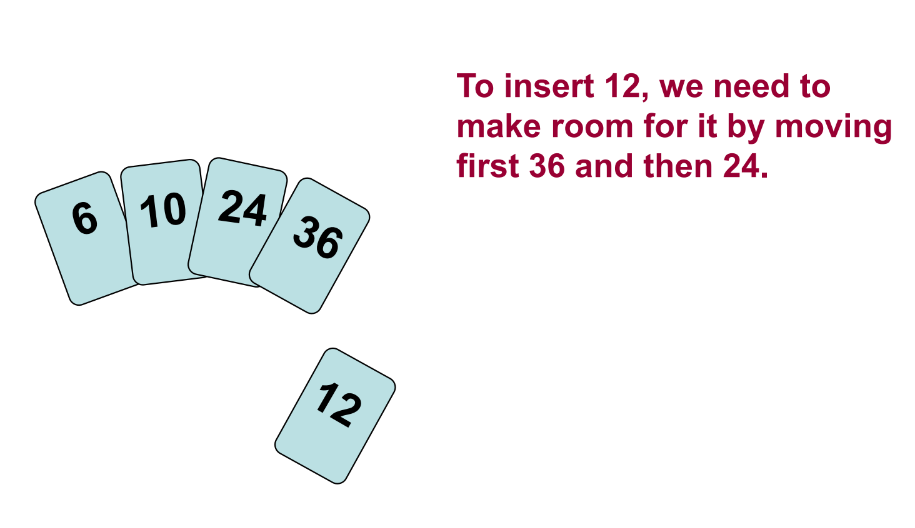
\includegraphics[width=0.7\textwidth]{assets/ins1.png}
        \caption{Caption for Step 1}
    \end{figure}
\end{frame}

\begin{frame}{Insertion Sort - Step 2}
    \begin{figure}
        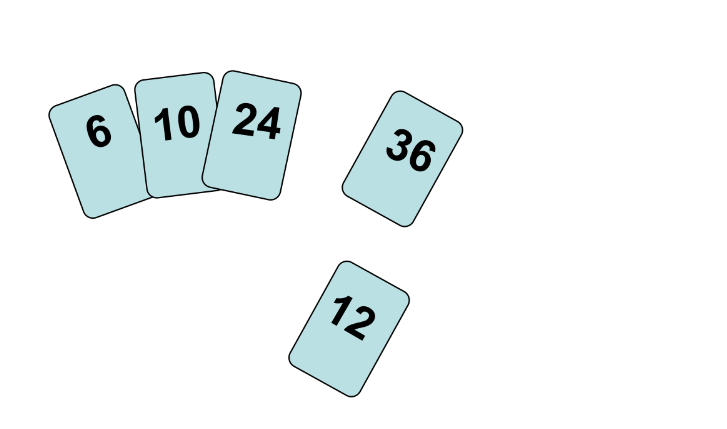
\includegraphics[width=0.7\textwidth]{assets/ins2.png}
        \caption{Caption for Step 2}
    \end{figure}
\end{frame}

\begin{frame}{Insertion Sort - Step 3}
    \begin{figure}
        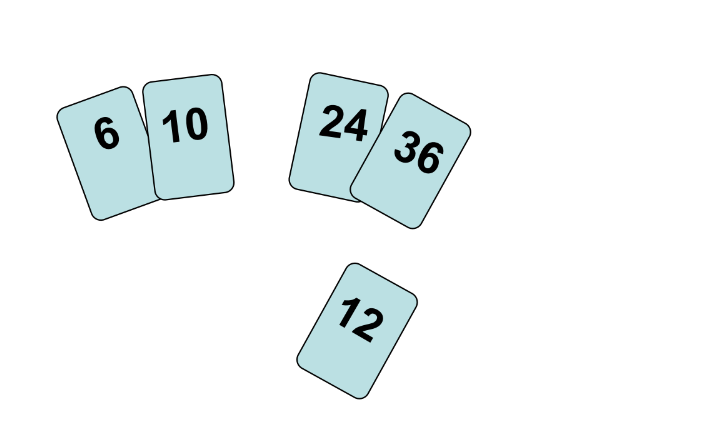
\includegraphics[width=0.7\textwidth]{assets/ins3.png}
        \caption{Caption for Step 3}
    \end{figure}
\end{frame}

\begin{frame}{Insertion Sort Example}
    \begin{figure}
        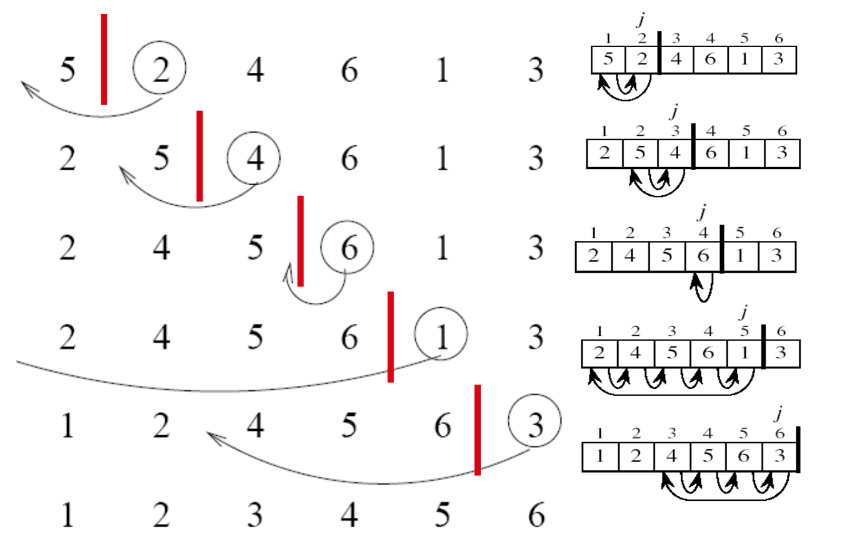
\includegraphics[width=0.7\textwidth]{assets/ins4.png}
        \caption{Caption for Step 4}
    \end{figure}
\end{frame}

\begin{frame}{Insertion Sort Example}
\vspace{1cm}
\begin{tabular}{|c|c|c|c|c|c|c|c|}
\hline
$A[0]$ & $A[1]$ & $A[2]$ & $A[3]$ & $A[4]$ & $A[5]$ & $A[6]$\\
\hline
$-\infty$ &\cellcolor{orange} $5$ & $2$ & $4$ & $6$ & $1$ & $3$ \\
\hline
\end{tabular}
\vspace{1cm}
\begin{table}[!hbt]
\begin{tabular}{|c|}
\hline key\\
\hline $5$\\
\hline
\end{tabular}\hspace{1cm}
%
\begin{tabular}{|c|c|c|c|c|c|c|c|}
\hline
$A[0]$ & $A[1]$ & $A[2]$ & $A[3]$ & $A[4]$ & $A[5]$ & $A[6]$\\
\hline
$-\infty$ &\cellcolor{orange} $5$ & $2$ & $4$ & $6$ & $1$ & $3$ \\
\hline
\end{tabular}
\end{table}
\begin{tikzpicture}
 {\hspace{3cm}} \draw[->, red, bend right=35] (3,0) to (6,0);
\end{tikzpicture}


\begin{tabular}{|c|c|c|c|c|c|c|c|}
\hline
$A[0]$ & $A[1]$ & $A[2]$ & $A[3]$ & $A[4]$ & $A[5]$ & $A[6]$\\
\hline
$-\infty$ &\cellcolor{statalegreen} $5$ & $2$ & $4$ & $6$ & $1$ & $3$ \\
\hline
\end{tabular}

\end{frame}


\begin{frame}{Insertion Sort Example}
\vspace{1cm}
\begin{tabular}{|c|c|c|c|c|c|c|c|}
\hline
$A[0]$ & $A[1]$ & $A[2]$ & $A[3]$ & $A[4]$ & $A[5]$ & $A[6]$\\
\hline
$-\infty$ &\cellcolor{yellow} $5$ &\cellcolor{orange} $2$ & $4$ & $6$ & $1$ & $3$ \\
\hline
\end{tabular}
\vspace{1cm}
\begin{table}[!hbt]
\begin{tabular}{|c|}
\hline key\\
\hline $2$\\
\hline
\end{tabular}\hspace{1cm}
%
\begin{tabular}{|c|c|c|c|c|c|c|c|}
\hline
$A[0]$ & $A[1]$ & $A[2]$ & $A[3]$ & $A[4]$ & $A[5]$ & $A[6]$\\
\hline
$-\infty$ & $5$ &\cellcolor{orange} $5$ & $4$ & $6$ & $1$ & $3$ \\
\hline
\end{tabular}
\end{table}
\begin{tikzpicture}
 {\hspace{3cm}} \draw[->, red, bend right=35] (3,0) to (5.8,0);
\end{tikzpicture}


\begin{tabular}{|c|c|c|c|c|c|c|c|}
\hline
$A[0]$ & $A[1]$ & $A[2]$ & $A[3]$ & $A[4]$ & $A[5]$ & $A[6]$\\
\hline
$-\infty$ & \cellcolor{statalegreen}$2$ &\cellcolor{statalegreen} $5$ & $4$ & $6$ & $1$ & $3$ \\
\hline
\end{tabular}

\end{frame}

\begin{frame}{Insertion Sort Example}
\vspace{1cm}
\begin{tabular}{|c|c|c|c|c|c|c|c|}
\hline
$A[0]$ & $A[1]$ & $A[2]$ & $A[3]$ & $A[4]$ & $A[5]$ & $A[6]$\\
\hline
$-\infty$ & $2$ &\cellcolor{yellow} $5$ &\cellcolor{orange} $4$ & $6$ & $1$ & $3$ \\
\hline
\end{tabular}
\vspace{1cm}
\begin{table}[!hbt]
\begin{tabular}{|c|}
\hline key\\
\hline $4$\\
\hline
\end{tabular}\hspace{1cm}
%
\begin{tabular}{|c|c|c|c|c|c|c|c|}
\hline
$A[0]$ & $A[1]$ & $A[2]$ & $A[3]$ & $A[4]$ & $A[5]$ & $A[6]$\\
\hline
$-\infty$ & $2$ & $5$ &\cellcolor{orange} $5$ & $6$ & $1$ & $3$ \\
\hline
\end{tabular}
\end{table}
\begin{tikzpicture}
 {\hspace{3cm}} \draw[->, red, bend right=30] (3,0) to (7,0);
\end{tikzpicture}


\begin{tabular}{|c|c|c|c|c|c|c|c|}
\hline
$A[0]$ & $A[1]$ & $A[2]$ & $A[3]$ & $A[4]$ & $A[5]$ & $A[6]$\\
\hline
$-\infty$ &\cellcolor{statalegreen} $2$ &\cellcolor{statalegreen} $4$ & \cellcolor{statalegreen}$5$ & $6$ & $1$ & $3$ \\
\hline
\end{tabular}

\end{frame}

\begin{frame}{Insertion Sort Example}
\vspace{1cm}
\begin{tabular}{|c|c|c|c|c|c|c|c|}
\hline
$A[0]$ & $A[1]$ & $A[2]$ & $A[3]$ & $A[4]$ & $A[5]$ & $A[6]$\\
\hline
$-\infty$ & $2$ & $4$ & $5$ &\cellcolor{orange} $6$ & $1$ & $3$ \\
\hline
\end{tabular}
\vspace{1cm}
\begin{table}[!hbt]
\begin{tabular}{|c|}
\hline key\\
\hline $6$\\
\hline
\end{tabular}\hspace{1cm}
%
\begin{tabular}{|c|c|c|c|c|c|c|c|}
\hline
$A[0]$ & $A[1]$ & $A[2]$ & $A[3]$ & $A[4]$ & $A[5]$ & $A[6]$\\
\hline
$-\infty$ & $2$ & $4$ & $5$ &\cellcolor{orange} $6$ & $1$ & $3$ \\
\hline
\end{tabular}
\end{table}
\begin{tikzpicture}
 {\hspace{3cm}} \draw[->, red, bend right=25] (3,0) to (9,0);
\end{tikzpicture}


\begin{tabular}{|c|c|c|c|c|c|c|c|}
\hline
$A[0]$ & $A[1]$ & $A[2]$ & $A[3]$ & $A[4]$ & $A[5]$ & $A[6]$\\
\hline
$-\infty$ & \cellcolor{statalegreen}$2$ & \cellcolor{statalegreen}$4$ & \cellcolor{statalegreen}$5$ & \cellcolor{statalegreen}$6$ & $1$ & $3$ \\
\hline
\end{tabular}

\end{frame}

\begin{frame}{Insertion Sort Example}
\vspace{1cm}
\begin{tabular}{|c|c|c|c|c|c|c|c|}
\hline
$A[0]$ & $A[1]$ & $A[2]$ & $A[3]$ & $A[4]$ & $A[5]$ & $A[6]$\\
\hline
$-\infty$ & \cellcolor{yellow}$2$ &\cellcolor{yellow} $4$ &\cellcolor{yellow} $5$ &\cellcolor{yellow} $6$ &\cellcolor{orange} $1$ & $3$ \\
\hline
\end{tabular}
\vspace{1cm}
\begin{table}[!hbt]
\begin{tabular}{|c|}
\hline key\\
\hline $1$\\
\hline
\end{tabular}\hspace{1cm}
%
\begin{tabular}{|c|c|c|c|c|c|c|c|}
\hline
$A[0]$ & $A[1]$ & $A[2]$ & $A[3]$ & $A[4]$ & $A[5]$ & $A[6]$\\
\hline
$-\infty$ & $2$ & $2$ & $4$ & $5$ &\cellcolor{orange} $6$ & $3$ \\
\hline
\end{tabular}
\end{table}
\begin{tikzpicture}
 {\hspace{3cm}} \draw[->, red, bend right=35] (3,0) to (5.8,0);
\end{tikzpicture}


\begin{tabular}{|c|c|c|c|c|c|c|c|}
\hline
$A[0]$ & $A[1]$ & $A[2]$ & $A[3]$ & $A[4]$ & $A[5]$ & $A[6]$\\
\hline
$-\infty$ & \cellcolor{statalegreen}$1$ & \cellcolor{statalegreen}$2$ &\cellcolor{statalegreen} $4$ & \cellcolor{statalegreen}$5$ & \cellcolor{statalegreen}$6$ & $3$ \\
\hline
\end{tabular}

\end{frame}

\begin{frame}{Insertion Sort Example}
\vspace{1cm}
\begin{tabular}{|c|c|c|c|c|c|c|c|}
\hline
$A[0]$ & $A[1]$ & $A[2]$ & $A[3]$ & $A[4]$ & $A[5]$ & $A[6]$\\
\hline
$-\infty$ & $1$ & $2$ &\cellcolor{yellow} $4$ &\cellcolor{yellow} $5$ &\cellcolor{yellow} $6$ &\cellcolor{orange} $3$ \\
\hline
\end{tabular}
\vspace{1cm}
\begin{table}[!hbt]
\begin{tabular}{|c|}
\hline key\\
\hline $3$\\
\hline
\end{tabular}\hspace{1cm}
%
\begin{tabular}{|c|c|c|c|c|c|c|c|}
\hline
$A[0]$ & $A[1]$ & $A[2]$ & $A[3]$ & $A[4]$ & $A[5]$ & $A[6]$\\
\hline
$-\infty$ & $1$ & $2$ & $4$ & $4$ & $5$ &  \cellcolor{orange}$6$ \\
\hline
\end{tabular}
\end{table}
\begin{tikzpicture}
 {\hspace{3cm}} \draw[->, red, bend right=25] (3,0) to (8,0);
\end{tikzpicture}


\begin{tabular}{|c|c|c|c|c|c|c|c|}
\hline
$A[0]$ & $A[1]$ & $A[2]$ & $A[3]$ & $A[4]$ & $A[5]$ & $A[6]$\\
\hline
$-\infty$ & \cellcolor{statalegreen}$1$ & \cellcolor{statalegreen}$2$ &\cellcolor{statalegreen}$3$&\cellcolor{statalegreen} $4$ & \cellcolor{statalegreen}$5$ & \cellcolor{statalegreen}$6$  \\
\hline
\end{tabular}

\end{frame}

\begin{frame}{Insertion Sort Algorithm}
    
    \begin{algorithm}[H]
        \caption{Insertion Sort}
        \begin{algorithmic}[1]
            \Procedure{InsertionSort}{$\text{arr}[ ]$, $\text{n}$}
                \For{$\text{i} \gets 1$ to $\text{n}$}
                    \State $\text{key} \gets \text{arr}[\text{i}]$
                    \State $\text{j} \gets \text{i} - 1$
                    \While{$\text{j} \geq 0$ and $\text{key} < \text{arr}[\text{j}]$}
                        \State $\text{arr}[\text{j} + 1] \gets \text{arr}[\text{j}]$
                        \State $\text{j} \gets \text{j} - 1$
                    \EndWhile
                    \State $\text{arr}[\text{j} + 1] \gets \text{key}$
                \EndFor
            \EndProcedure
        \end{algorithmic}
    \end{algorithm}
\end{frame}

\begin{frame}[fragile]{Insertion Sort in C++}
    \begin{lstlisting}[style=cppStyle]
void insertionSort(int arr[],int n) {
    for (int i = 1; i < n; ++i) {
        int key = arr[i];
        int j = i - 1;

        while (j >= 0 && array[j] > key) {
            arr[j + 1] = arr[j];
            --j;
        }

        arr[j + 1] = key;
    }
}
    \end{lstlisting}
\end{frame}

\begin{frame}{Time and Space Complexity of Insertion Sort}
    The time complexity of Insertion Sort varies under different scenarios.

    \begin{itemize}
        \item \textbf{Best Case:} When the array is already sorted, the algorithm only needs to compare each element with its predecessor, requiring $n$ steps to sort the $n$-element array. The number of comparisons is limited to $n$, resulting in linear time complexity.
        
        \item \textbf{Worst Case:} In the worst case, when the array is reverse-sorted, Insertion Sort has to insert each element at the beginning of the sorted subarray, resulting in a time complexity of $O(n^2)$.
        
        \item \textbf{Average Case:} In the average case, where the array elements are in random order, the running time is approximately $O(n^2 / 4) = O(n^2)$. Since every element must be compared to every other element, $(n-1)$ comparisons are conducted for every nth element. Consequently, $n \cdot (n-1)$ is the total number of comparisons.
    \end{itemize}

    Regarding space complexity, Insertion Sort uses a constant amount of additional variables besides the input array, resulting in a space complexity of $O(1)$.
\end{frame}



\subsection{Quick Sort Algorithm}

\begin{frame}{Quick Sort Introduction}
    Quick Sort is a highly efficient sorting algorithm that uses a divide-and-conquer strategy to sort an array.\cite{5}
    It works by selecting a "pivot" element from the array and partitioning the other elements into two sub-arrays according to whether they are less than or greater than the pivot. The sub-arrays are then recursively sorted.
    
    The key steps in the Quick Sort algorithm include selecting a pivot, partitioning the array, and recursively applying the Quick Sort to the sub-arrays. 
\end{frame}

\begin{frame}{Partition Function - Working Principle}
    \textbf{Choose a pivot:} In general, the first element, a random element, or the last element of the sample is selected as the pivot.

    \textbf{Set up pointers:} Two pointers, named low and high, are initialized at the beginning and end of the array that is going to be partitioned.

    \textbf{Iterate and swap:} The algorithm iterates through the array, comparing elements with the pivot and swapping them based on the following rules:
    \begin{itemize}
        \item If an element at low is larger than or equal to the pivot, swap it with the element at high and decrement high.
        \item Otherwise, increment low.
    \end{itemize}

    \textbf{Place pivot in position:} When the low and high pointers meet, swap the pivot with the element at high. This places the pivot in its final sorted position, with smaller elements to its left and larger elements to its right. Also, return the index of high as it is needed in the main algorithm to find the particular index.
\end{frame}

\begin{frame}{Idea of Quick Sort Algorithm}
    \begin{figure}
        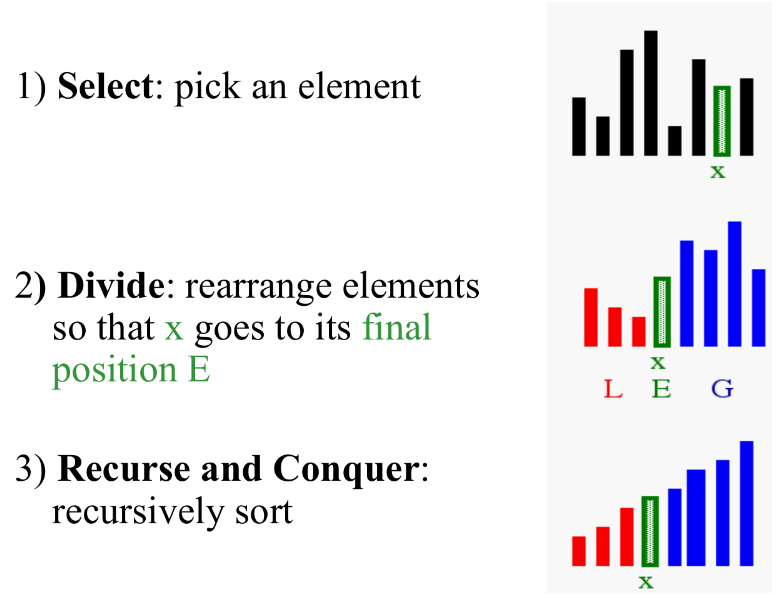
\includegraphics[width=0.6\textwidth]{assets/idea.png}
        \caption{Caption for Idea of Quick}
    \end{figure}
\end{frame}



\begin{frame}{QuickSort Example: Given Array}
  \begin{itemize}
    \item Given array: $a[7] = \{5, 7, 6, 1, 3, 2, 4\}$
  \end{itemize}
\end{frame}

\begin{frame}{QuickSort: Choosing a Pivot and Partitioning (Steps 1-2)}
  \begin{columns}
    \begin{column}{0.4\textwidth}
      \begin{itemize}
        \item Choose a pivot: $\text{pivot} = 4$ (last element)
        \item Original array: $\{5, 7, 6, 1, 3, 2, 4\}$
        \item After partitioning: $\{1,3,2, \textbf{4}, 7,6,5\}$
        \item Left subarray: $\{1,3,2\}$ \item Right subarray: $\{7,6,5\}$
      \end{itemize}
    \end{column}
    \begin{column}{0.6\textwidth}
      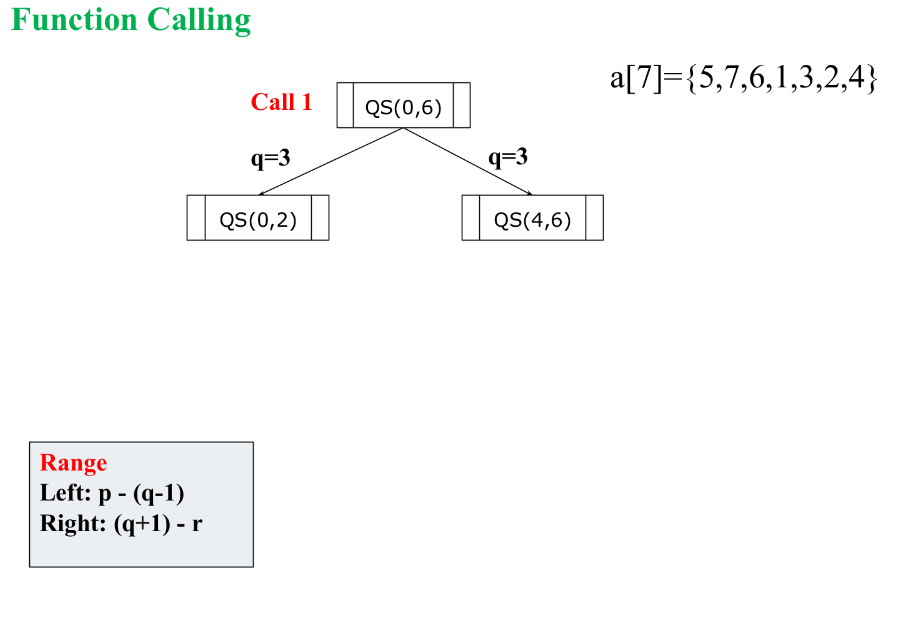
\includegraphics[width=1\textwidth]{assets/Qu1.png}
    \end{column}
  \end{columns}
\end{frame}

\begin{frame}{QuickSort: Recursion on Left Subarray (Steps 3-4)}
  \begin{columns}
    \begin{column}{0.4\textwidth}
      \begin{itemize}
        \item Left subarray: $\{1,3,2\}$
        \item Choose pivot: $\text{pivot} = 2$ (last element)
        \item After partitioning: $\{1, 2, 3\}$
      \end{itemize}
    \end{column}
    \begin{column}{0.6\textwidth}
      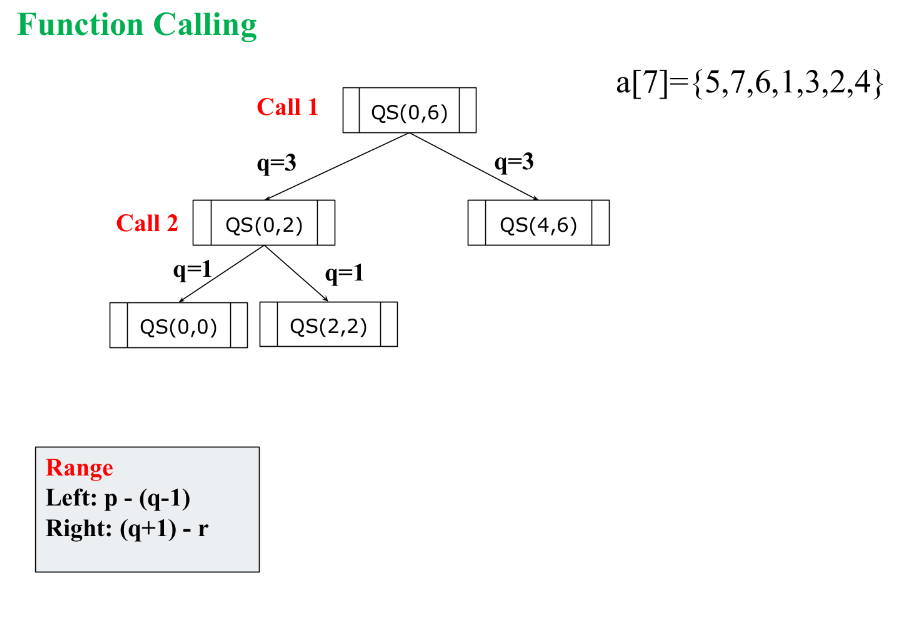
\includegraphics[width=\textwidth]{assets/Qu2.png}
    \end{column}
  \end{columns}
\end{frame}



\begin{frame}{QuickSort: Recursion on Right Subarray (Steps 5-6)}
  \begin{columns}
    \begin{column}{0.4\textwidth}
      \begin{itemize}
        \item Right subarray: $\{7,6,5\}$
        \item Choose pivot: $\text{pivot} = 5$ (last element)
        \item After partitioning: $\{ \textbf{5},6, 7\}$
      \end{itemize}
    \end{column}
    \begin{column}{0.6\textwidth}
      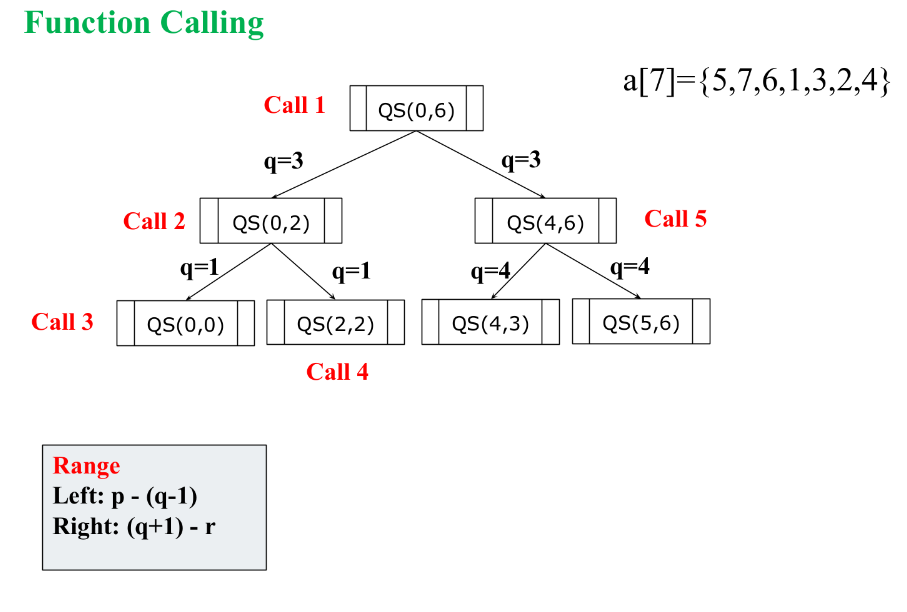
\includegraphics[width=\textwidth]{assets/Qu3.png}
    \end{column}
  \end{columns}
\end{frame}

\begin{frame}{QuickSort: Combine Sorted Subarrays (Step 7)}
  \begin{columns}
    \begin{column}{0.4\textwidth}
      \begin{itemize}
        \item Combine sorted subarrays: $\{1, 2, 3, 4, 5, 6, 7\}$
      \end{itemize}
    \end{column}
    \begin{column}{0.6\textwidth}
      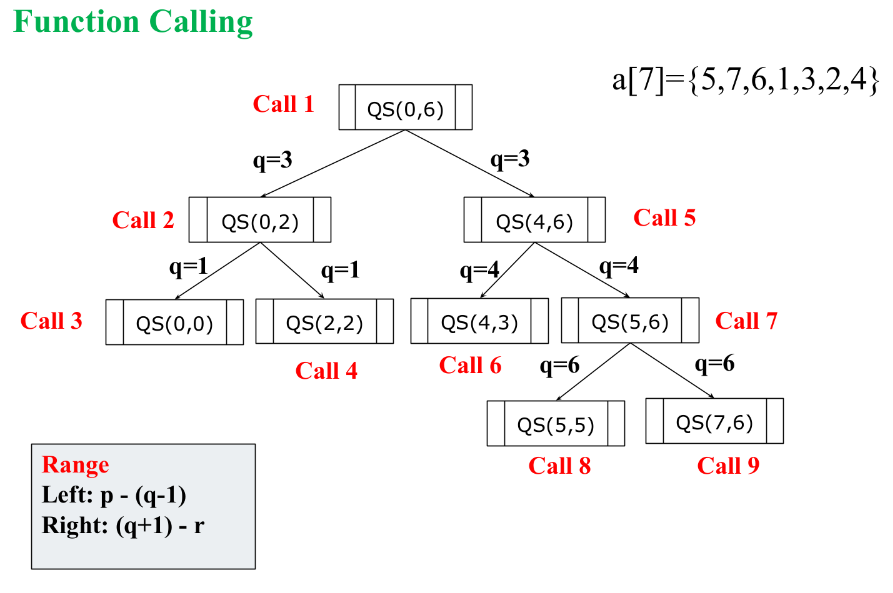
\includegraphics[width=\textwidth]{assets/Qu4.png}
    \end{column}
  \end{columns}
\end{frame}





\begin{frame}{Quick Sort Algorithm}
    \begin{algorithm}[H]
        \caption{Quick Sort}
        \begin{algorithmic}[1]
            \Procedure{QuickSort}{$\text{arr}[ ]$, $\text{low}$, $\text{high}$}
                \If{$\text{low} < \text{high}$}
                    \State $\text{pivot} \gets \text{Partition}(\text{arr}, \text{low}, \text{high})$
                    \State $\text{QuickSort}(\text{arr}, \text{low}, \text{pivot} - 1)$
                    \State $\text{QuickSort}(\text{arr}, \text{pivot} + 1, \text{high})$
                \EndIf
            \EndProcedure
        \end{algorithmic}
    \end{algorithm}
\end{frame}



\begin{frame}{Partition Function}
    \begin{algorithm}[H]
        \caption{Partition}
        \begin{algorithmic}[1]
            \Function{Partition}{$\text{arr}[ ]$, $\text{low}$, $\text{high}$}
                \State $\text{pivot} \gets \text{arr}[\text{high}]$
                \State $\text{i} \gets \text{low} - 1$
                \For{$\text{j} \gets \text{low}$ \textbf{to} $\text{high} - 1$}
                    \If{$\text{arr}[\text{j}] \leq \text{pivot}$}
                        \State Swap $\text{arr}[\text{i+1}]$ and $\text{arr}[\text{j}]$
                        \State $\text{i} \gets \text{i} + 1$
                    \EndIf
                \EndFor
                \State Swap $\text{arr}[\text{i+1}]$ and $\text{arr}[\text{high}]$
                \State \textbf{return} $\text{i+1}$
            \EndFunction
        \end{algorithmic}
    \end{algorithm}
\end{frame}



\begin{frame}[fragile]{Quick Sort Function in C++}
    \begin{lstlisting}[style=cppStyle]
void quickSort(int arr[], int low, int high) {
    if (low < high) {
        int pivot = partition(arr, low, high);

        quickSort(arr, low, pivot - 1);
        quickSort(arr, pivot + 1, high);
    }
}
    \end{lstlisting}
\end{frame}

\begin{frame}[fragile]{Partition Function in C++}
    \begin{lstlisting}[style=cppStyle]
int partition(int arr[], int low, int high) {
    int pivot = arr[high];
    int i = (low - 1);

    for (int j = low; j <= high - 1; ++j) {
        if (arr[j] < pivot) {
            swap(arr[i+1], arr[j]);
            i++;
        }
    }

    swap(arr[i + 1], arr[high]);

    return (i + 1);
}
    \end{lstlisting}
\end{frame}



\begin{frame}{Time and Space Complexity of Quick Sort}
    Quick Sort has good average-case performance and is often faster in practice compared to other sorting algorithms.

    \begin{itemize}
        \item \textbf{Best Case:} The best-case time complexity is $O(n \log n)$ when the partitioning is balanced.
        
        \item \textbf{Worst Case:} The worst-case time complexity is $O(n^2)$, but this occurs infrequently in practice. Choosing a good pivot strategy helps avoid the worst-case scenario.
        
        \item \textbf{Average Case:} On average, Quick Sort has a time complexity of $O(n \log n)$.
        \cite{1}\cite{6}\cite{7}
    \end{itemize}

    Quick Sort typically uses $O(\log n)$ additional space for the recursive call stack, resulting in a space complexity of $O(\log n)$. However, in the worst case, it can use $O(n)$ additional space if the partitioning is highly unbalanced.
\end{frame}

\begin{frame}{Best Case Time Complexity - Mathematical Detail (Part 1)}
    \textbf{Best Case Recurrence Relation:}
    \[ T(N) = 2 \cdot T\left(\frac{N}{2}\right) + N \cdot \text{constant} \]

    \textbf{Solving the Recurrence:}
    \begin{align*}
        T(N) &= 2 \cdot \left(2 \cdot T\left(\frac{N}{4}\right) + \frac{N}{2} \cdot \text{constant}\right) + N \cdot \text{constant} \\
        &= 4 \cdot T\left(\frac{N}{4}\right) + 2 \cdot \text{constant} \cdot N
    \end{align*}
\end{frame}
\begin{frame}{Best Case Time Complexity - Mathematical Detail (Part 2)}
    Generalizing this pattern, we get:
    \[ T(N) = 2^k \cdot T\left(\frac{N}{2^k}\right) + k \cdot \text{constant} \cdot N \]

    Setting \(2^k = N\) and solving for \(k\), we get \(k = \log_2 N\).

    Substituting this back into the equation, we find:
    \[ T(N) = N \cdot T(1) + N \cdot \log_2 N \cdot \text{constant} \]

    Therefore, the best-case time complexity is \(O(N \log N)\).
\end{frame}
\begin{frame}{Average Case Time Complexity - Mathematical Detail (Part 1)}
    \textbf{Average Case Recurrence Relation:}
    \[ T(N) = \frac{2}{N} \sum_{i=1}^{N-1} T(i) \]

    \textbf{Solving the Recurrence:}
    \begin{align*}
        N \cdot T(N) &= 2 \sum_{i=1}^{N-1} T(i) \\
        (N-1) \cdot T(N-1) &= 2 \sum_{i=1}^{N-2} T(i)
    \end{align*}
\end{frame}
\begin{frame}{Average Case Time Complexity - Mathematical Detail (Part 2)}
    Subtracting the second equation from the first:
    \[ N \cdot T(N) - (N-1) \cdot T(N-1) = (N + 1) \cdot T(N-1) + 2 \cdot N \cdot \text{constant} \]

    Simplifying, we get:
    \[ T(N) = \frac{\log_2 N \cdot (N + 1)}{2} \]

    Therefore, the average-case time complexity is \(O(N \log N)\).
\end{frame}
\begin{frame}{Worst Case Time Complexity - Mathematical Detail (Part 1)}
    \textbf{Worst Case Recurrence Relation:}
    \[ T(N) = T(N - 1) + N \cdot \text{constant} \]

    \textbf{Solving the Recurrence:}
    \begin{align*}
        T(N) &= T(N - 1) + N \cdot \text{constant} \\
        &= T(N - 2) + (N - 1) \cdot \text{constant} + N \cdot \text{constant} \\
        &= T(N - 3) + 2 \cdot N \cdot \text{constant} - \text{constant} \\
        & \ \vdots \\
        &= T(N - k) + k \cdot N \cdot \text{constant} - \frac{k \cdot (k - 1)}{2} \cdot \text{constant}
    \end{align*}
\end{frame}

\begin{frame}{Worst Case Time Complexity - Mathematical Detail (Part 2)}
    If we put \(k = N\), then:
    \begin{align*}
        T(N) &= T(0) + N^2 \cdot \text{constant} - \frac{N \cdot (N-1)}{2} \cdot \text{constant} \\
        &= \frac{N^2}{2} + \frac{N}{2}
    \end{align*}

    Therefore, the worst-case time complexity is \(O(N^2)\).
\end{frame}



